\documentclass[12pt,a4paper,final]{extreport}
\usepackage[utf8]{inputenc}
\usepackage{amsmath}
\usepackage{bm}
\usepackage{amsfonts}
\usepackage{fancyhdr}
\usepackage[algo2e]{algorithm2e} 
\usepackage{amssymb}
\usepackage{float}
\usepackage{placeins}
\usepackage{graphicx}
\usepackage[left=2.5cm,right=2.5cm,top=2cm,bottom=2cm]{geometry}
\linespread{1.2}
\usepackage{setspace}
\usepackage{titlesec}
\usepackage[yyyymmdd]{datetime}

\usepackage{times}
\renewcommand{\bibname}{REFERENCES}
\usepackage{enumerate}
\usepackage{etoolbox}
\patchcmd{\chapter}{plain}{empty}{}{}

\usepackage{tocloft,calc}
\renewcommand{\cftchappresnum}{\chaptername\space}
\setlength{\cftchapnumwidth}{\widthof{\textbf{Appendix~999~}}}
\makeatletter
\g@addto@macro\appendix{%
  \addtocontents{toc}{%
    \protect\renewcommand{\protect\cftchappresnum}{\appendixname\space}%
  }%
}
\makeatother

\titleformat{\chapter}[display]
{\normalfont\rmfamily\large\bfseries}
{\chaptertitlename\ \thechapter \centering }{16pt}{\centering \huge\uppercase}
\renewcommand{\chaptername}{CHAPTER}{\Large}
\titleformat{\section}
{\normalfont\rmfamily\normalsize\bfseries}
{\thesection}{14pt}{\large}

 \titleformat{\subsection}
{\normalfont\rmfamily\small\bfseries}
{\thesubsection}{12pt}{\normalsize} 

 \titleformat{\subsubsection}
{\normalfont\rmfamily\small\bfseries}
{\thesubsection}{12pt}{\normalsize} 

\titlespacing{\chapter}{0pc}{0pc}{0.5pc}
\titlespacing{\section}{0pc}{.5pc}{0pc}
\titlespacing{\subsection}{0pc}{1pc}{0pc}
\thispagestyle{empty}


\author
{   \textbf{Ganesh Sekhar (CHN16CS)}\\
	\textbf{Shan Eapen Koshy (CHN16CS)} \\[0.1mm]
	\textbf{Sachin Sajan Punoose (CHN16CS)} \\[0.1mm]
	\textbf{S Hemanth (CHN16CS098)} \\[0.1mm]
	\textbf{to}\\
 }
\title{{\Large\textbf{Generating Usability Reports from User Inputs and Eye Movements}} \\
\vspace{1.2cm}	{\large\textbf{A PROJECT REPORT}}\\[0.2cm]
	{\small submitted by}
		}
\date{\begin{center}
\begin{small}
The APJ Abdul Kalam Technological University\\
in partial fulfillment of the requirements for the award of the Degree\\[0.2cm]
of\\[0.2cm]
Bachelor of Technology\\[0.2cm]
In\\[0.2cm]
\textit{Computer Science and Engineering}\\\end{small}
\begin{figure}[h]	
\begin{center}

\includegraphics[scale=0.3]{ceclogo.png} \\[.1cm]
\end{center}
\end{figure}
	\textbf{ Department of Computer Science and Engineering} \\
	 College of Engineering, Chengannur, Kerala -689121\\	
	July 2020\end{center}
}	

\begin{document}
\pagenumbering{gobble}
\clearpage\maketitle

\section*{\begin{center} \fontsize{14}{17} \selectfont \textbf{DECLARATION}\end{center}}
\begin{quote}

We undersigned hereby declare that the project report "Generating Usability Reports from User Inputs and Eye Movements", submitted for partial fulfillment of the requirements for the award of degree of Bachelor of Technology of the APJ Abdul Kalam Technological University, Kerala is a bonafide work done by us under supervision of Ms.Angel, Assistant Professor. This submission represents our ideas in our own words and where ideas or words of others have been included, We have adequately and accurately cited and referenced the original sources. We also declare that we have adhered to ethics of academic honesty and integrity and have not misrepresented or fabricated any data or idea or fact or source in my submission. We understand that any violation of the above will be a cause for disciplinary action by the institute and/or the University and can also evoke penal action from the sources which have thus not been properly cited or from whom proper permission has not been obtained. This report has not been previously formed the basis for the award of any degree, diploma or similar title of any other University.

\begin{tabbing}
\hspace{8.8cm}\=\kill
Place: CHENGANNUR  \> Ganesh Sekhar \\  Date:\today  \>Shan Eapen Koshy \\ \hspace{8.8cm} Sachin Sajan Punnoose \\ \hspace{8.8Cm} S Hemanth
\end{tabbing} 
\end{quote}
\newpage
\clearpage
\thispagestyle{empty}

\begin{center}\fontsize{14}{17} \selectfont \textbf{DEPARTMENT OF COMPUTER SCIENCE AND ENGINEERING}\end{center}
\begin{center}\fontsize{14}{17} \selectfont \textbf{COLLEGE OF ENGINEERING,CHENGANNUR}\end{center}
%\begin{center}\fontsize{14}{17} \selectfont \textbf{PALAKKAD}\end{center}
\begin{figure}[h]
	\begin{center}
		
\includegraphics[scale=.33]{ceclogo.png}
		\vspace{.1 cm}
	\end{center}
\end{figure}

\begin{center}\fontsize{14}{17} \selectfont \textbf{CERTIFICATE}\end{center}
This is to certify that the report entitled \textbf{{\large "Generating Usability Reports from User Inputs and Eye Movements"}} submitted by \textbf{Ganesh Sekhar}, \textbf{Shan Eapen Koshy}, \textbf{Sachin Sajan Punnoose}, \textbf{S Hemanth} to the APJ Abdul Kalam Technological University in partial fulfillment of the requirements for the award of the Degree of Bachelor of Technology in Department of Computer Science and Engineering, College of Engineering, Chengannur, Kerala -689121 is a bonafide record of the project work carried out by them under my/our guidance and supervision. This report in any form has not been submitted to any other University or Institute for any purpose.

\vspace{2cm}
\vspace{2cm}
\begin{flushleft}
	\hspace{0.1cm}\textbf{Ms. Angel Thankam Thomas} \hspace{6.4cm}\textbf{Ms.Shiny B }\\
	\hspace{0.1cm}Assistant Professor \hspace{8.5cm}Assistant Professor\\
	\hspace{0.1cm}Project Guide \hspace{9.4cm}Project Co-ordinator
	
\end{flushleft}
\vspace{0.5cm}
\begin{center}
\textbf{Dr. Smitha Dharan}\\Professor and Head	
\end{center}




\newpage
\pagenumbering{roman}
\addcontentsline{toc}{chapter}{ACKNOWLEDGEMENT}
\section*{\begin{center} \fontsize{14}{17} \selectfont \textbf{ACKNOWLEDGEMENT}\end{center}}


%\vspace{.4 cm }
\begin{quote}
{
    First and foremost we wish to express our wholehearted indebtedness to God Almighty for his gracious constant care and blessings showered over us for the successful completion of this project.\par
	\hspace{01 cm}We are deeply indebted to \textbf{Dr. Jacob Thomas V}, Principal, College of Engineering, Chengannur and Associate Professor \textbf{Dr. Smitha Dharan}, Head of the Department of Computer Science and Engineering, College of Engineering, Chengannur, for providing and availing all the required facilities for undertaking the project in a systematic way.\par
	\hspace{01 cm}We would like to express my deep gratitude to our Project Co-ordinator \textbf{Ms.Shiny B}, Assistant Professor, for the incite and encouragement given by her to improve the project. We are thankful to our guide \textbf{Ms. Angel Thankam Thomas}, Assistant Professor for providing good suggestions and valuable advices to improve the project.\par
	\hspace{01 cm}Gratitude is extended to all teaching and non teaching staffs of Department of Computer Science and Engineering, College of Engineering, Chengannur, for the sincere directions imparted and the cooperation in connection with the project.\par
	\hspace{01 cm}We are also thankful to our parents for the support given in connection with the project. Gratitude may be extended to all well-wishers and friends who supported us.
	\begin{flushright}
Ganesh Sekhar\\
Shan Eapen Koshy\\
Sachin Sajan Punnoose\\
S Hemanth
\end{flushright}
}
\end{quote}


\newpage
\section*{\begin{center} \fontsize{14}{17} \selectfont \textbf{ABSTRACT}\end{center}}

\addcontentsline{toc}{chapter}{ABSTRACT}
\begin{quote}
    Usability testing is a technique used to evaluate a product by testing it on users. It is an important factor in marketing a product since it gives a complete structure of how the users use the product.

    After understanding how real users interact with your product, you can improve the product based on the results. The primary purpose of a usability test is to improve it’s designed so as to make it more user-friendly.
    
    The proposed system uses eye detection to locate the positions on the screen where the user pays more attention and a heat map is generated from it. This testing is done for different age groups and a final report listing all the findings (positives and negatives) is generated. Positive findings will help the team to know that they’re on the right track and the negative findings provide proposals to solve them
    


\end{quote}

\newpage
\tableofcontents
\addtocontents{toc}{\small}


\newpage
\listoffigures 
\addtocontents{toc}{\small}
\addcontentsline{toc}{chapter}{LIST OF FIGURES}

\clearpage
\pagenumbering{arabic}
%\pagestyle{fancy}
\lhead{\textit{Generating Usability Reports from User Inputs and Eye Movements}}
\chead{}
\rhead{}
\lfoot{\textit{College of Engineering,Chengannur}}
\cfoot{}
\rfoot{\thepage}
\renewcommand{\headrulewidth}{0.4pt}
\renewcommand{\footrulewidth}{0.4pt}
\pagestyle{fancy}


%%%%%%%%%%%%%%%%%%%%%%%%%%%%%%%%%%%%%%%%%%%%%%%%%%%%%%%%%%%%%%%%%%%%%%%%

\chapter{INTRODUCTION}
\vspace{0.3cm}
\noindent
Usability Testing is defined as a type of software testing where, a small set of target endusers,
of a software system, ”use” it to expose usability defects. This testing mainly focuses
on the user’s ease to use the application, flexibility in handling controls and the ability of the
system to meet its objectives. It is also called User Experience(UX) Testing.
Eye tracking provides compelling objective data that reveals the human behaviour behind
the interaction with interfaces or products and uncovers optimization potential. User Experience
(UX) and Human-Computer Interaction (HCI) researchers have been recognizing the
unique value of eye tracking for a long time and it is now more than ever available to be easily
integrated in innovation processes.
Traditional usability methods and performance measurements might indicate that there’s an
efficiency issue, but often do not answer why or how to fix it. Eye tracking uniquely provides
information about tasks that aren’t articulated by participants and that might otherwise pass unobserved
by the researcher. It captures natural, unbiased user behavior and produces objective
data to allow effective recommendations to be made. Eye tracking is a flexible technique that
works with a variety of research methods, including observations, interviews, and retrospective
think aloud (RTA).
Our approach combines eye tracking with several other data points such as cursor movements,
mouse clicks, hover duration and more to score the UI elements present in the screen to
generate an interactive report.


\vspace{0.5cm}
\newpage
\chapter{PROBLEM FORMULATION}
\vspace{0.3cm}
Usability testing is crucial in a software development life cycle as it provides more insights
on how a user uses the product. Typically, a UX researcher summons the tester to his/her office
and has to manually observe and analyze the user to validate the designs. But this traditional
usability testing approach takes huge amount of time, money and workforce. This in turn
increases the software development time which causes late delivery of the product. Different
usability testing metrics that UX designers uses are:
\begin{itemize}
    \item Focus points of the users on the screen
    \item Time taken by the user to find the target action/data he/she was looking for
    \item Session duration
\end{itemize}
To find the focus points, the UX researcher asks the tester to move a pointer across the
screen which is prone to errors. The other metrics are also manually recorded which are prone
to errors. To overcome this we propose a novel method to automate usability testing that accounts
various other metrics including eye tracking.


\newpage
\chapter{LITERATURE REVIEW}
\section{Eye-Tracking}
\subsection{TurkerGaze}
\paragraph{}
Turkergaze introduces a webcam-based gaze tracking system that supports large-scale, crowdsourced eye tracking deployed on Amazon Mechanical Turk. By a combination of careful algorithm and gaming protocol design, our system obtains eye tracking data for saliency prediction comparable to data gathered in a traditional lab setting, with relatively lower cost and less effort on the part of the researchers.
The main disadvantage with TurkerGaze is that the calibration time is quite high and comes with limited browser support.
\subsection{XLabsGaze}
\paragraph{}
xLabsGaze is a webcam based eye tracking technology that comes with it's own pros and cons. It offers realtime tracking without restricting user movement. Once thoroughly calibrated, it just works all the time, allowing users to get up and sit down as much as they like. The main downside to XLabsGaze is that it requires the web developer to send the video feed to their server for eye tracking which can be slow and also pose privacy concerns. They also offer a C++ SDK and chrome plugin but that doesn't provide the web accessibility that we need.
\subsection{WebGazer.js}
\paragraph{}
WebGazer.js is also an eye tracking library that uses common webcams to infer the eye-gaze locations of web visitors on a page in real time. The eye tracking model it contains self-calibrates by watching web visitors interact with the web page and trains a mapping between the features of the eye and positions on the screen.

\section{Usability Testing}
\subsection{Eye Tracking in User Experience Testing: How to Make the Most of It}
\paragraph{}
As eye tracking technology becomes more precise, affordable, and unobtrusive, its popularity continues to increase among usability practitioners. This paper introduces eye tracking as a user experience testing tool. It focuses on how to design and conduct studies involving eye tracking, so that eye movement data can effectively supplement data obtained through more conventional methods. Using examples from actual studies, It lessons learned and provide advice on how to avoid common mistakes.


\newpage
\chapter{PROPOSED SYSTEM}
\paragraph{}
In this proposed system, a user can submit a URL of the website to be analyzed. The system then generates a unique tracking code for this website which can be manually inserted into the website to be tested.
Testers can access this URL and interact with the website normally while we collect the tester's eye coordinates that we obtained through webgazer.js. Basic demographic of the tester such as age and gender are also collected for categorization and report generation. The collected data is then stored in the server. 
The testing details can be reviewed from the admin's dashboard. Several features such as timeline, demographic filtering, heatmap,AOI, etc, are provided for easily analyzing the data.
\begin{figure}[H]
    \centering
    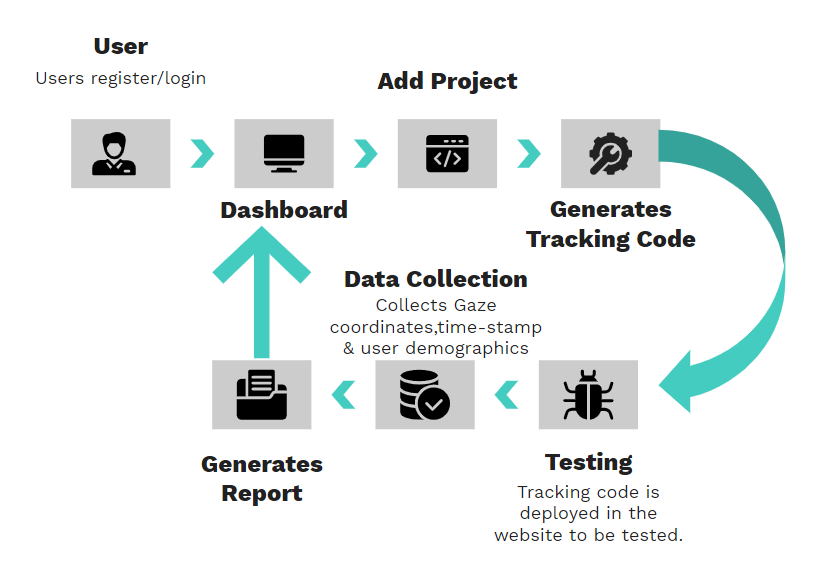
\includegraphics[width=\linewidth]{proposed-method.png}
    \counterwithin{figure}{section}
    \caption{Control Flow Diagram}
\end{figure}
The system mainly consist of 2 parts:
\begin{itemize}
	\item Client Side Script
	\item Backend \& Dashboard
\end{itemize}
\section{Client Side Script}
This consist of various module that are exectude int the client side.This module is responsible for the calibration and the optimization of testers eye movements \& sending the eye tracking data along with the user demographic to the server for further processing.

It mainly consist of the following modules:
\subsection{Tracking Script}
The functionality of the tracking Script is similar to that of the Google Analytics Tracking code. This script enables our service to track the users website. For each websites a unique tracking script is generated and the script is inserted into the \textbf{\textit{head}} tag of the website to be tested.
\begin{figure}[H]
    \centering
    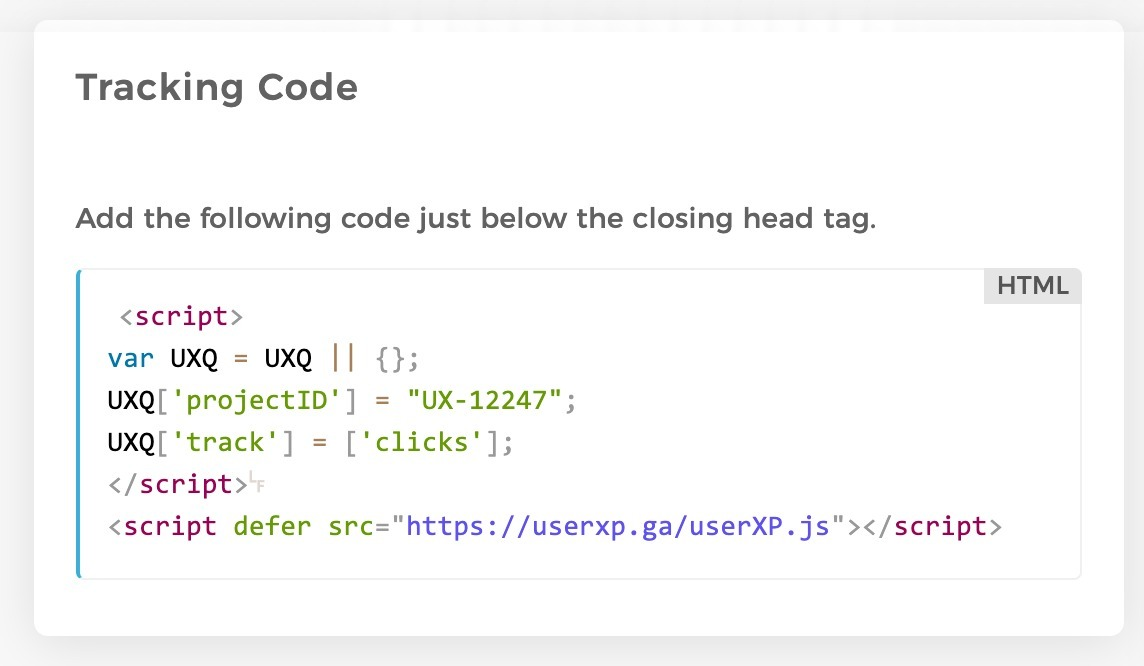
\includegraphics[width=\linewidth]{tracking-script.png}
    \counterwithin{figure}{section}
    \caption{Tracking Script}
\end{figure}

\subsection{Callibration \& Eye Tracking}
When the website to be tested is loaded it's content is replaced by the callibration page. During the calibration process the system learns how a tester’s eyes move when they are looking at certain parts of the screen.
WebGazer, a self callibrated eye-tracking library is used for obtaining the eye-gaze locations of varoius testers on the website in real time.

In the initial phase of callibration the eye tracking model is self callibrated by matching the pupil positions and eye features with screen locations during user interactions.
After the calibration process, the users website is reloaded and the testers interact with it just like any other website for a time period of 30sec. Then the tester fills up a form regarding the tester demographics and this data along with the tracking data is updated into the server.
\begin{figure}[H]
    \centering
    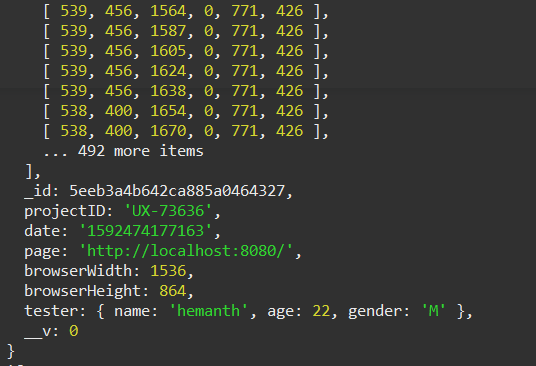
\includegraphics[width=\linewidth]{tracking-data.png}
    \counterwithin{figure}{section}
    \caption{Tracking Data}
\end{figure}

The above figure shows a snippet of the data being posted to the server after the test.
The submited data consist the following data:
\begin{itemize}
	\item Project ID: A unique ID to identify each project.
	\item URL: URL of the website to be tested.
	\item Browser Dimentions: It consist of the browser width and height in pixels.
	\item User Demographics: Details such as name, age and gender of the tester.
	\item Gaze-Recording: It consist of 5 attributes-Eye Coordinates(both x \& y coordinates), Timestamp, Scroll Offset and Mouse Coordinates(both x \& y coordinates) respectively.
\end{itemize}

\subsection{Dashboard}

It's an interactive website made using HTML,CSS \& JS which acts as platform for the users for adding,managing and the deletion of their projects.
Each of the projects page is equipped with various details such as tracking code, user demographic chart and the listing of all the testers along with the report.

\textbf{dashboard Pic?}
\newpage
\section{Backend}
The backend of our service uses NodeJs, EJS Templating and Mongodb for the database.
NodeJs was used due to its high performance and the due to the fact that client side script is written in javascript so less time learning a different language.

EJS or Embedded Javascript Templating is a simple templating engine used by NodeJs that lets you generate HTML markup with plain JavaScript.It can inject data into HTML template at the client side and produce the final HTML. It is used because of it's fast compilation and rendering property.
EJS also support Js on the server side and is also supported by all the browsers.

Mongodb is leading NoSQl, cross-platform, document oriented database that provides, high performance, high availability, and easy scalability. MongoDB works on concept of collection and document. The data is stored in BSON(Binary JSON) format in the form of key-value pair.

\textbf{Sample mongodb record pic?}

\newpage
\chapter{HOW IT WORKS?}


\newpage
\chapter{FEATURES OF USABILITY REPORT}

\newpage
\chapter{PROBLEMS WE FACED}

\newpage
\chapter{CONCLUSION }
\paragraph{}
At present, existing Usability\-Testing methods for web based platforms are quite expensive and requires a considerable amount of resources including man-power and time.
Thus to overcome these challenges, the proposed system uses eye-tracking, cursor-movement and mouse-clicks to evaluate the positions on the screen where the user pays more attention and a score for each UI element is assigned from the resulting heat-map.
This testing is done for different age groups a final analysis report is generated. The UX team in turn can use this report to identify what they have done right \& wrong and hence improve their design.The default behavior of EJS is that it looks into the ‘views’ folder for the templates to render. So all the webpages required is to be stored in the views folder in ejs format.


\newpage
\addcontentsline{toc}{chapter}{REFERENCES}
\vspace{0.3cm}
\begin{thebibliography}{}
    \bibitem{1}
    Papoutsaki, Alexandra \& Sangkloy, Patsorn \& Laskey, James \& Daskalova, Nediyana \& Huang, Jeff \& Hays, James. (2016). \emph{WebGazer: Scalable Webcam Eye Tracking Using User Interactions.}
    \bibitem{d}
    Kiril Alexiev, Teodor Toshkov and Peter Dojnow. 2019. Accuracy and Precision of eye tracker by head movement compensation and calibration. \emph{20th International Conference on Computer Systems and Technologies
    (CompSysTech'19)}, Jun 21-22, 2019, Ruse, Bulgaria, 8 pages.
    https://doi.org/10.1145/3345252.3345278.

\end{thebibliography}

\end{document}

